\newtheorem{definition}{Definition}[section]
%\newtheorem{corollary}{Corollary}[definition]
\newtheorem{lemma}[definition]{Lemma}

\chapter{Einführung}

Als Einstieg in das Thema \textit{Kostenminimale Flüsse} soll das folgende Szenario betrachtet werden:\\
Ein Logistikunternehmen muss von seinen Verteilzentren aus mehrere Verkaufsstandorte eines Kunden beliefern. Es existieren verschiedene Routen, welche sich jedoch in ihrer Kapazität sowie ihren Kosten (z.B. Fahrzeit oder Spritkosten, bedingt durch den jeweiligen Kraftstoffverbrauch) unterscheiden. Wie soll der Logistiker die LKWs leiten, um unter Berücksichtigung der Kapazitäten den besten Weg zu finden? \\
Das Szenario ist exemplarisch in Abbildung \ref{fig:baeckerbeispiel} dargestellt.

\begin{figure}[htb]
\centering
\includegraphics[width=0.9\textwidth]{img/philipp/Bäckerbeispiel.pdf}
\caption{Logistik Beispiel \cite[vgl.][]{buesing2010graphen}}
\label{fig:baeckerbeispiel}
\end{figure}

Durch Anwendung des Wissens über die \textit{kürzesten Wege}, würde man nun von jedem Verteilzentrum zu jedem Verkaufsstandort den kürzesten Weg suchen. Anschließend müssten für jeden Verkaufsstandort nur noch aus den verfügbaren Wegen der jeweilige kürzeste Weg ausgewählt werden. Dieser Ansatz mag zwar in vielen Fällen funktionieren, jedoch existieren in der Realität häufig Einschränkungen, welche nicht einfach vernachlässigt werden können. Skaliert man das Szenario nämlich einmal hoch, hat man statt 5 möglicherweise 200 LKWs. Eine Route durch das kleine Wohngebiet mit einspuriger Straße würde zwar zunächst am schnellsten erscheinen - dieser Vorteil verschwindet jedoch, wenn statt der üblichen paar Autos plötzlich 200 LKWs durch das Wohngebiet fahren möchten. Eine Verteilung über verschiedene Routen würde dieses Problem umgehen.

Das Ziel ist somit, dass innerhalb eines \textit{Netzwerks} Wege von einem oder mehreren Startpunkten hin zu einem oder mehreren Zielen gefunden werden müssen. Dabei sind neben der Streckenkapazität weitere Bedingungen zu beachten:
\begin{enumerate}
    \item Die Verteilzentren, formal \textit{Quellen} genannt, haben ein limitiertes Angebot. In diesem Beispiel hat die linke Quelle zwei LKWs und die rechte drei.
    \item Die Verkaufsstandorte, formal \textit{Senken} genannt, haben eine begrenzte Nachfrage. In diesem Beispiel benötigt der mittlere Standort eine Einheit, die anderen zwei.
\end{enumerate}

Es ist schnell festzustellen, dass die genannten Probleme eine Mischung aus den bereits behandelten Themen darstellen: Einerseits sollen Kapazitätsbedingungen erfüllt werden, was die Verteilung hoher Lasten erfordert und aus \enquote{Maximale Flüsse} bekannt ist. Dazu kommen die Herausforderungen von \enquote{Kürzeste Wege}, da auch in diesem Thema die Kosten minimiert werden sollen.

% Einführung muss folgendem entsprechen: Kostenminimale Wege =  "Kostengünstigten Weg unter Beachtung der Kapaziätsgrenzen mit dem Ziel, dass die Balancen gleich null sind"

\newpage

\section{Wiederholung}

Für das bessere Verständnis und um Missverständnisse bei der Notation vorzubeugen, sollen zunächst die grundlegenden Aspekte der Themen \enquote{Kürzeste Wege} und \enquote{Maximale Flüsse} wiederholt werden. 

\subsection{Kürzeste Wege}

Kürzeste Wege haben das Ziel, den kürzesten bzw. ressourcenärmsten Weg zwischen zwei Knoten zu bestimmen.

\begin{definition}
    Sei $G = (V,E)$ ein Digraph (gerichteter Graph) mit einer Kantenbewertung $c(e) \geq 0$ für jede Kante $e \in E$ und seien $s, t \in V$ zwei Knoten (s für engl. source und t für engl. target). Ein (s, t)-Weg in $G$ heißt kürzester Weg, falls sein Gewicht verglichen mit dem Gewicht jedes anderen (s, t)-Wegs minimal ist. Das Gewicht $c(p)$ eines Wegs $p$ ist definiert als
    \begin{equation}
        c(p) = \displaystyle\sum_{e \in p}^{} c(e).
    \end{equation}
\end{definition}

Somit entspricht das Gewicht eines Weges dem kumulierten Gewicht der zugehörigen Kanten. Ist ein Weg ein kürzester Weg eines Graphen, so existiert kein anderer Weg mit einem geringeren Gewicht. Nimmt man nun einen Teilweg $(s', t')$ dieses Weges, so ist auch dies der kürzeste Weg:
\begin{lemma}
Sei $p$ ein kürzester (s, t)-Weg. Dann ist jeder zusammenhängende Teilweg von $p$ ein kürzester Weg.
\end{lemma}

\begin{figure}[ht]
\centering
\includegraphics[width=0.7\textwidth]{img/philipp/graph1-kürzeste Wege.drawio.pdf}
\caption{Beispiel für kürzeste Wege}
\label{fig:shortestpath}
\end{figure}
In Abbildung \ref{fig:shortestpath} ist ein Beispiel gegeben, bei dem jede Kante durch Kantenkosten beschrieben wird. Die dick markierten Kanten bilden den kürzesten Weg von Knoten $s$ zu Knoten $z$ ab. Es ist zu erkennen, dass obiges Lemma auch hier gilt und somit jeder Teilweg des kürzesten Weges $(s,z)$ ein kürzester Weg ist: So ist der Teilweg $(c,z)$ von $(s,z)$ der kürzeste Weg vom Knoten $c$ zum Knoten $z$.

\subsection{Maximale Flüsse}

Maximale Flüsse haben das Ziel, den größtmöglichen Fluss bzw. den höchsten Transport von einem Quellknoten zu einem Zielknoten herzustellen.

\begin{definition}
    Sei $G = (V,E)$ ein gerichteter Graph mit oberen Kapazitäten $u(e)$ für jede Kante $e \in E$ und zwei markierte Knoten $s, t \in V$ (kurz: Netzwerk (G, u, s, t)). Ein (s, t)-Fluss ist eine Kantenbewertung $f : E \to R \geq 0$, die die Kantenkapazitäten einhält und für die an jedem Knoten $v \in V \setminus \{s, t\}$ Flusserhaltung gilt. 
\end{definition}

Die genannte Definition enthält einige neue Begriffe, die nachfolgend nochmal differenziert werden.
    
Ein (s, t)- Fluss f hält die Kantenkapazitäten ein, wenn gilt:
\begin{equation}
    f(e) \leq u(e) \quad \forall e \in E.
\end{equation}
D.h. dass an einer Kante mit der Kapazität 5 auch nur maximal 5 Einheiten fließen können. Während ein realer, natürlicher Fluss ohne Probleme überlaufen kann, würde dies hier einen Widerspruch zur Definition bzw. einen instabilen Zustand erreichen.

An einem Knoten $v \in V$ liegt Flusserhaltung vor, wenn
\begin{equation}
    \displaystyle\sum_{e \in \delta ^{+} (v)}^{} f(e) - \displaystyle\sum_{e \in \delta ^{-} (v)}^{} f(e) = 0
    \label{formular:flusserhaltung}
\end{equation}
Mit $\delta ^{-}$ werden die eingehenden Kanten in $v$ bezeichnet und mit $\delta ^{+}$ die ausgehenden Kanten. Somit gilt die Flusserhaltung, wenn ein Knoten genau so viele Einheiten aufnimmt, wie er auch wieder abgibt\footnote{Zu beachten: Hier wird sich auf den tatsächlichen Fluss und nicht auf die Kapazitäten bezogen}.\\
An dieser Stelle ist festzustellen, dass die Flusserhaltung für Quellen und Senken nur dann gelten kann, wenn der (s,t)-Fluss den Wert 0 hat.

Der Wert (engl. value) eines (s, t)-Flusses ist definiert durch:
\begin{equation}
    \textrm{value}(f) = \displaystyle\sum_{e \in \delta ^{+} (s)}^{} f(e) - \displaystyle\sum_{e \in \delta ^{-} (s)}^{} f(e)
    \label{formular:flusswert}
\end{equation}
Beispiel: Schickt eine Quelle 5 Einheiten in das Netz und nimmt selber 2 Einheiten auf, so hat der Fluss den Wert 3. Dies ist damit zu begründen, dass die wieder aufgenommenen Einheiten ebenfalls der Quelle entstammen und damit der tatsächliche Fluss bzw. die Anzahl Einheiten, die am Ziel ankommen können, geringer ist.\\
Alternativ zur Betrachtungsweise, worin der Fokus auf der Quelle liegt, kann auch die Senke betrachtet werden, da die Anzahl an Einheiten, welche Quelle emittiert und Senke aufnimmt, gleich sein muss (zumindest bei einem Graphen mit einer Quelle und einer Senke).

\begin{figure}[ht]
\centering
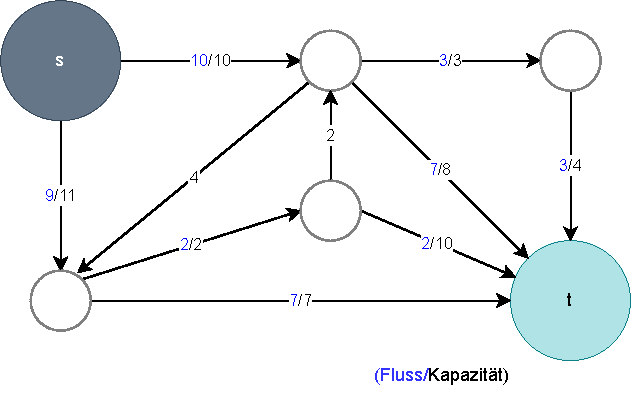
\includegraphics[width=0.7\textwidth]{img/philipp/graph1-Max Fluss.drawio.pdf}
\caption{Beispiel für maximale Flüsse}
\label{fig:maxfluss}
\end{figure}

In Abbildung \ref{fig:maxfluss} ist beispielhaft ein mögliches Maximale-Flüsse-Problem dargestellt. Jede Kante wird durch eine Kapazität und einen Flusswert beschrieben.\\
In diesem Fall hätte der maximale Fluss den Wert 19, d.h. dass in der angegebenen \textit{Kantenkonstellation} maximal 19 Einheiten zum Ziel fließen können.


\section{Definition \& Notation}

Nachdem die Vorgängerthemen nochmal wiederholt wurden, können nun die für \textit{kostenminimale Flüsse} benötigten Definitionen und Begriffe eingeführt werden.

\begin{definition}
    Sei $G = (V,E)$ ein gerichteter Graph mit oberen Kapazitäten $u(e)$ für jede Kante $e \in E$ und $b$ eine Balance. Ein b-Fluss ist eine Kantenbewertung $f(e), e \in E$, die die oberen Kapazitäten einhält und für die der Einfluss in einem Knoten $v$ abzüglich des Ausflusses in den Knoten $v$ dem Wert $b(v)$ entspricht, d.h. 
    \begin{equation}
        \displaystyle\sum_{e \in \delta ^{+} (v)}^{} f(e) - \displaystyle\sum_{e \in \delta ^{-} (v)}^{} f(e) = b(v)
    \end{equation}
\end{definition}

Die Formel der Flusserhaltung wurde somit um den Begriff der \textit{Balance} erweitert. Entsprechend gilt die Flusserhaltung bei einer Balance von Null. Durch diese Regel hat eine Quelle\footnote{welche mehr emittiert als aufnimmt} eine positive Balance und eine Senke\footnote{welche mehr aufnimmt als emittiert} eine negative Balance.

Unter Berücksichtigung des Wissens aus den \enquote{Maximalen Flüssen}, ist ein Ziel, die Balancen auf Null zu bekommen, also eine konsequente Flusserhaltung zu erzeugen. Damit dies möglich ist, kann die folgende Aussage angenommen werden:
\begin{equation*}
    \displaystyle\sum_{v \in V}^{} b(v) = 0
\end{equation*}
Diese Aussage sorgt nicht nur dafür, dass die Flusserhaltung überall eingehalten wird, sondern Angebot und Nachfrage von Quellen und Senken ausbalanciert sind.

Um die b-Flüsse untereinander vergleichen zu können, erfordert es einer neuen Metrik:

\begin{definition}
    Sei $G = (V,E)$ ein gerichteter Graph mit oberen Kapazitäten $u(e) \in \mathbb{N}$ und Kosten $c(e) \in \mathbb{Z}$ für jede Kante $e \in E$. Außerdem sei $b$ eine Balance. Ein kostenminimaler Fluss $f$ ist ein b-Fluss mit minimalen Kosten. Die Kosten eines b-Flusses sind gegeben durch
    \begin{equation}
        c(f) = \displaystyle\sum_{e \in E}^{} c(e) \cdot f(e)
    \end{equation}
\label{def:costfunktion}
\end{definition}

Anders formuliert, entsprechen Kostenminimale Wege dem kostengünstigten Weg unter Beachtung der Kapaziätsgrenzen mit dem Ziel, dass die Balancen gleich null sind.

\section{Erste Anwendung}
Angenommen, es liegt der aus dem Logistikbeispiel bekannte Graph vor (siehe Abbildung \ref{fig:baeckerbeispiel2}). In dieser Darstellung erhält jede Kante $v$ ein Kantengewicht $c(v)$ (grauer Wert) sowie eine Kapazität $f(v)$ (schwarzer Wert). Das Ziel ist es, dass bei dem mittleren Zielknoten $t2$ eine Einheit und bei den verbleibenden $t_x$ zwei Einheiten ankommen.

\begin{figure}[ht]
\centering
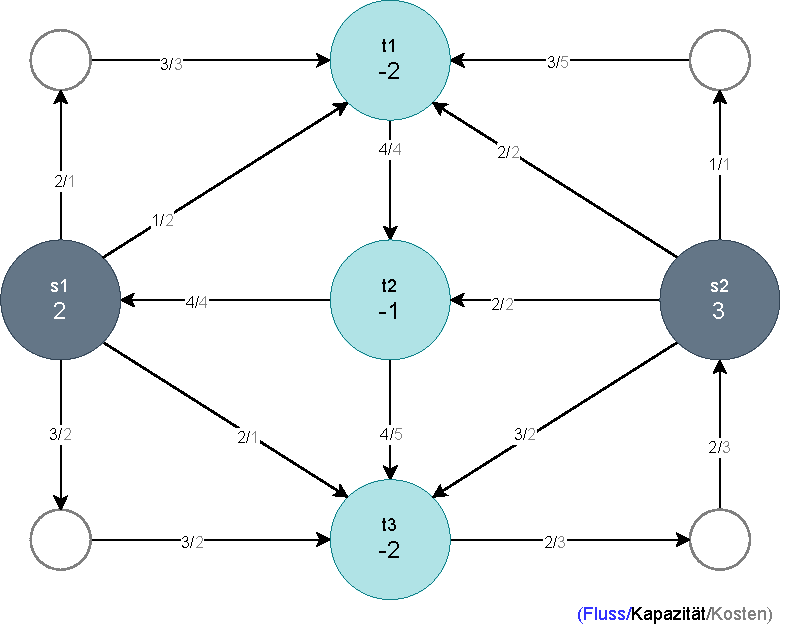
\includegraphics[width=0.7\textwidth]{img/philipp/graph1-example0.drawio.pdf}
\caption{Formelle Darstellung des Logistikbeispiels}
\label{fig:baeckerbeispiel2}
\end{figure}

Durch Ausprobieren lassen sich nun verschiedene Flüsse ermitteln, wie in den Abbildungen \ref{fig:baeckerbeispiel_loesungen1} und \ref{fig:baeckerbeispiel_loesungen2} exemplarisch zu sehen ist. Diese müssen nun lediglich auf ihr kumuliertes Kantengewicht überprüft werden. In diesem Fall hätte Möglichkeit 1 ein Gewicht von 5 und Möglichkeit 2 ein Gewicht von 6, womit die erste die \textit{kostenminimalere} ist.

\begin{figure}[htb]
\centering
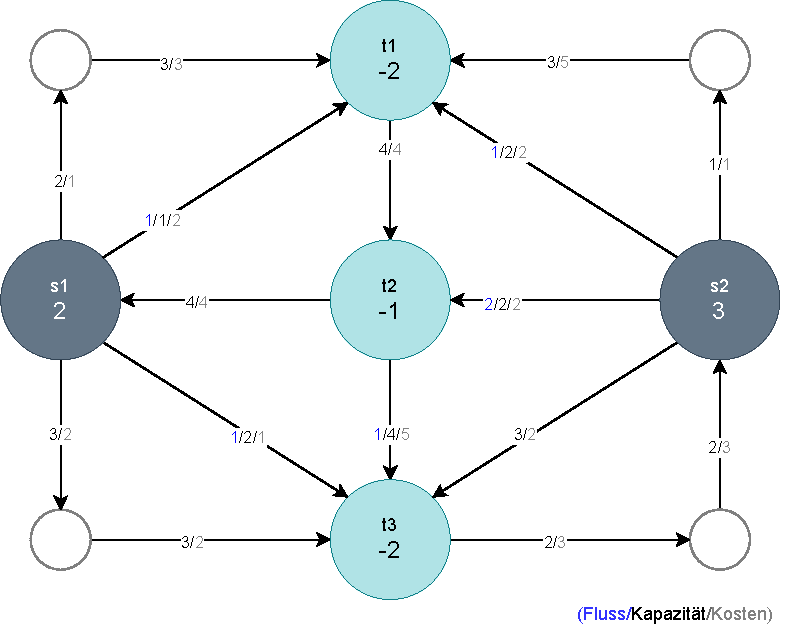
\includegraphics[width=0.7\textwidth]{img/philipp/graph1-example1.drawio.pdf}
\caption{1. Möglicher Fluss des Logistikbeispiels}
\label{fig:baeckerbeispiel_loesungen1}
\end{figure}

\begin{figure}[htb]
\centering
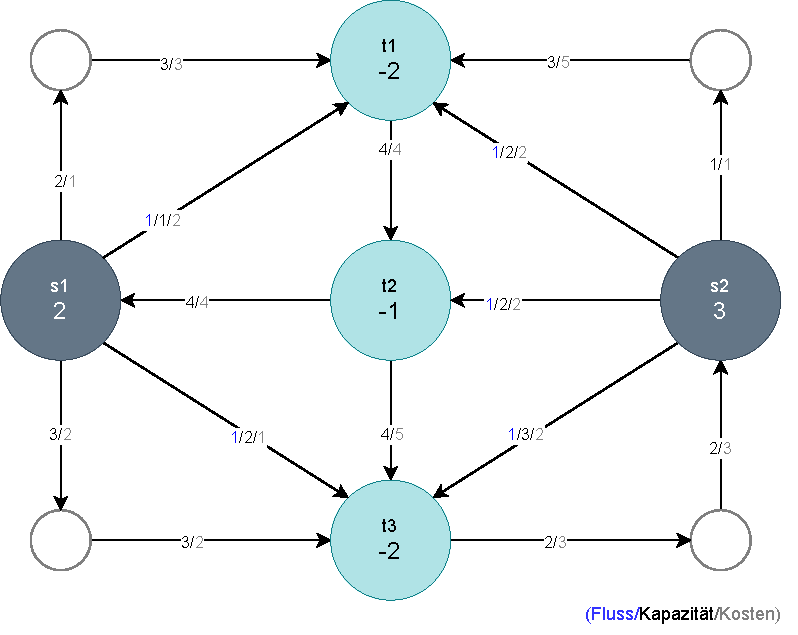
\includegraphics[width=0.7\textwidth]{img/philipp/graph1-example 2.drawio.pdf}
\caption{2. Möglicher Fluss des Logistikbeispiels}
\label{fig:baeckerbeispiel_loesungen2}
\end{figure}

Würde man nun, statt nur zwei, alle Möglichkeiten ausprobieren, wäre der Fluss mit dem geringsten Kantengewicht der gesuchte kostenminimale Fluss. \\
Bekanntermaßen ist eine Herangehensweise, in der alle möglichen Wege durchprobiert werden (vergleichbar zu \textit{BruteForce}) intuitiv, jedoch unverhältnismäßig ineffizient. Diese Ausarbeitung wird in den nächsten Kapiteln bessere Wege aufzeigen, um solche Probleme zu lösen. Hierzu wird sich eines Optimalitätskriteriums unter Anwendung der Residualgraphen bedient, die Thema des nächsten Kapitels sein werden.